\documentclass{article}
\usepackage{vmlmacros}
\usepackage{tikz}
\usepackage{float}
\floatstyle{boxed} 
\restylefloat{figure}


\title{Overview of our Languages}
\author{Roger Burtonpatel}
\date{November 24, 2023}
\begin{document}
\maketitle

\it{This document is meant as an accompaniment to the grammars presented in} \\
\tt{syntax-judgement-V-.pdf}\it{,} \\
\tt{syntax-judgement-P+.pdf}\it{, and} \\
\tt{decision-trees.pdf}\it{.}



\bigskip
\begin{figure}[H]
    \centering
    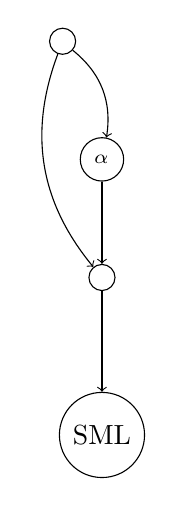
\begin{tikzpicture}
        \node[circle, draw] (1) at (5,5) {\Pplus};
        \node[circle, draw] (2) at (5.5,3.5) {$\Vminus_{\alpha}$};
        \node[circle, draw] (3) at (5.5,2) {\Dalpha};
        \node[circle, draw] (4) at (5.5,0) {SML};


        \draw[->] (1)[bend left] to (2);
        \draw[->] (2) to (3);
        \draw[->] (3) to (4);
        \draw[->] (1) to[bend right] (3);
    \end{tikzpicture}
    \caption{Flow of language translation.}
    \label{fig:graph}
\end{figure}

\section{The Three Languages}

The first of our languages is \Pplus. This is the language of patterns. We know
we can compile patterns into decision trees. Our next language is \Vminus, the
language of equations. This uses the decision making construct \it{if-fi} to
perform different operations based on the form of a value. 

Both of these languages theoretically can be compiled to our third language,
\D: the language of decision trees. 

\bigskip

\section{Language Structure}

The three langauges look similar: they each have value constructors and 
a 'decision-making construct' to deal with constructed data. In \Pplus, the 
construct is pattern-matching; in \Vminus, it is the guarded expression; 
in \D, it is the decision tree. 

Of note in both \Vminus and \D is that the 'decision-making construct' is 
annotated with an $\alpha$. This annotation gives us type flexibility on the 
right-hand side of the \it{terminating} case for each construct 
(\tt{$\rightarrow$ exp} in \Vminus and the match node in \D.) 

Because of the $\alpha$, the right-hand side becomes immaterial: we don't care
about what we're returning; we care about the decision-making construct that
gets us there. Whether it's a single value (ML-style) a sequence of values
(Verse-style), or even something else, the $\alpha$ represents \it{any} ultimate
result of "making a decision," and it's the ways in which we make decisions that
we truly care about examining. By making the return result both polymorphic and
abstract, we eschew the need to worry about its type and compatibility with
other results of otherwise-equivalent trees. 

\section{Translation and Equivalency}

We aim to translate $\Pplus$ to both $\Vminus$ and $\D$ (Figure 1). By showing both
languages can be translated to decision trees, we show both express a common
property: that evaluation at runtime does not backtrack, i.e., no individual
part of a value used to make decisions (called a \tt{scrutinee}) is examined
more than once. Showing \Vminus expresses this no-backtracking property (and, by
extension, the "no-logical-variables-at-runtime" property, is a core aim of this
work.)

The second important translation is from $\Vminus$ to \D. Recall the $\alpha$ from
earlier: the polymorphic abstract type in both $\galpha$ and $\Dalpha$ shows
an equivalence preserved by translation. 

\it{Rough- want to hack this out with you:} \\
The equivalence is this: final, returned right-hand sides of 'decision-making 
constructs' can be anything. 



\end{document}